\section{Methodology}

%\subsection{Quati beamline}

The development of advanced catalytic and electrochemical materials for sustainable energy conversion requires analytical methodologies capable of resolving structural, electronic, and chemical transformations under realistic operating conditions. In this context, the integration of synchrotron radiation techniques with purpose-designed experimental cells represents a step toward understanding and controlling complex physico-chemical processes. 

The QUATI (Quick X-Ray Absorption Spectroscopy for Time and Space Resolved Experiments) beamline at the Brazilian fourth-generation synchrotron light source Sirius provides an unique platform for such investigations \cite{Santiago2023}. Operated by the Laboratório Nacional de Luz Síncrotron within the Centro Nacional de Pesquisa em Energia e Materiais, Sirius delivers high brilliance and low emittance X-ray beams that enable advanced spectroscopic measurements with unprecedented temporal and spatial resolution. As shown in Figure \ref{quati}, the QUATI beamline is specifically designed for high-resolution X-ray absorption spectroscopy, and offers capabilities ideally suited for in-situ and operando investigations of catalytic systems for steam reforming of ethanol and electrochemical devices such as solid oxide fuel cells and solid oxide electrolysis cells.

X-ray absorption spectroscopy provides element-specific information on local atomic structure and configuration without requiring long-range order. The technique encompasses the near-edge region, known as X-ray absorption near edge structure (XANES), which is sensitive to oxidation state and coordination symmetry \cite{XU2024}, and the extended region, known as extended X-ray absorption fine structure (EXAFS), which yields quantitative information on interatomic distances, coordination numbers, and disorder parameters \cite{MALZER2021}. 

\begin{figure}[h]
    \centering
    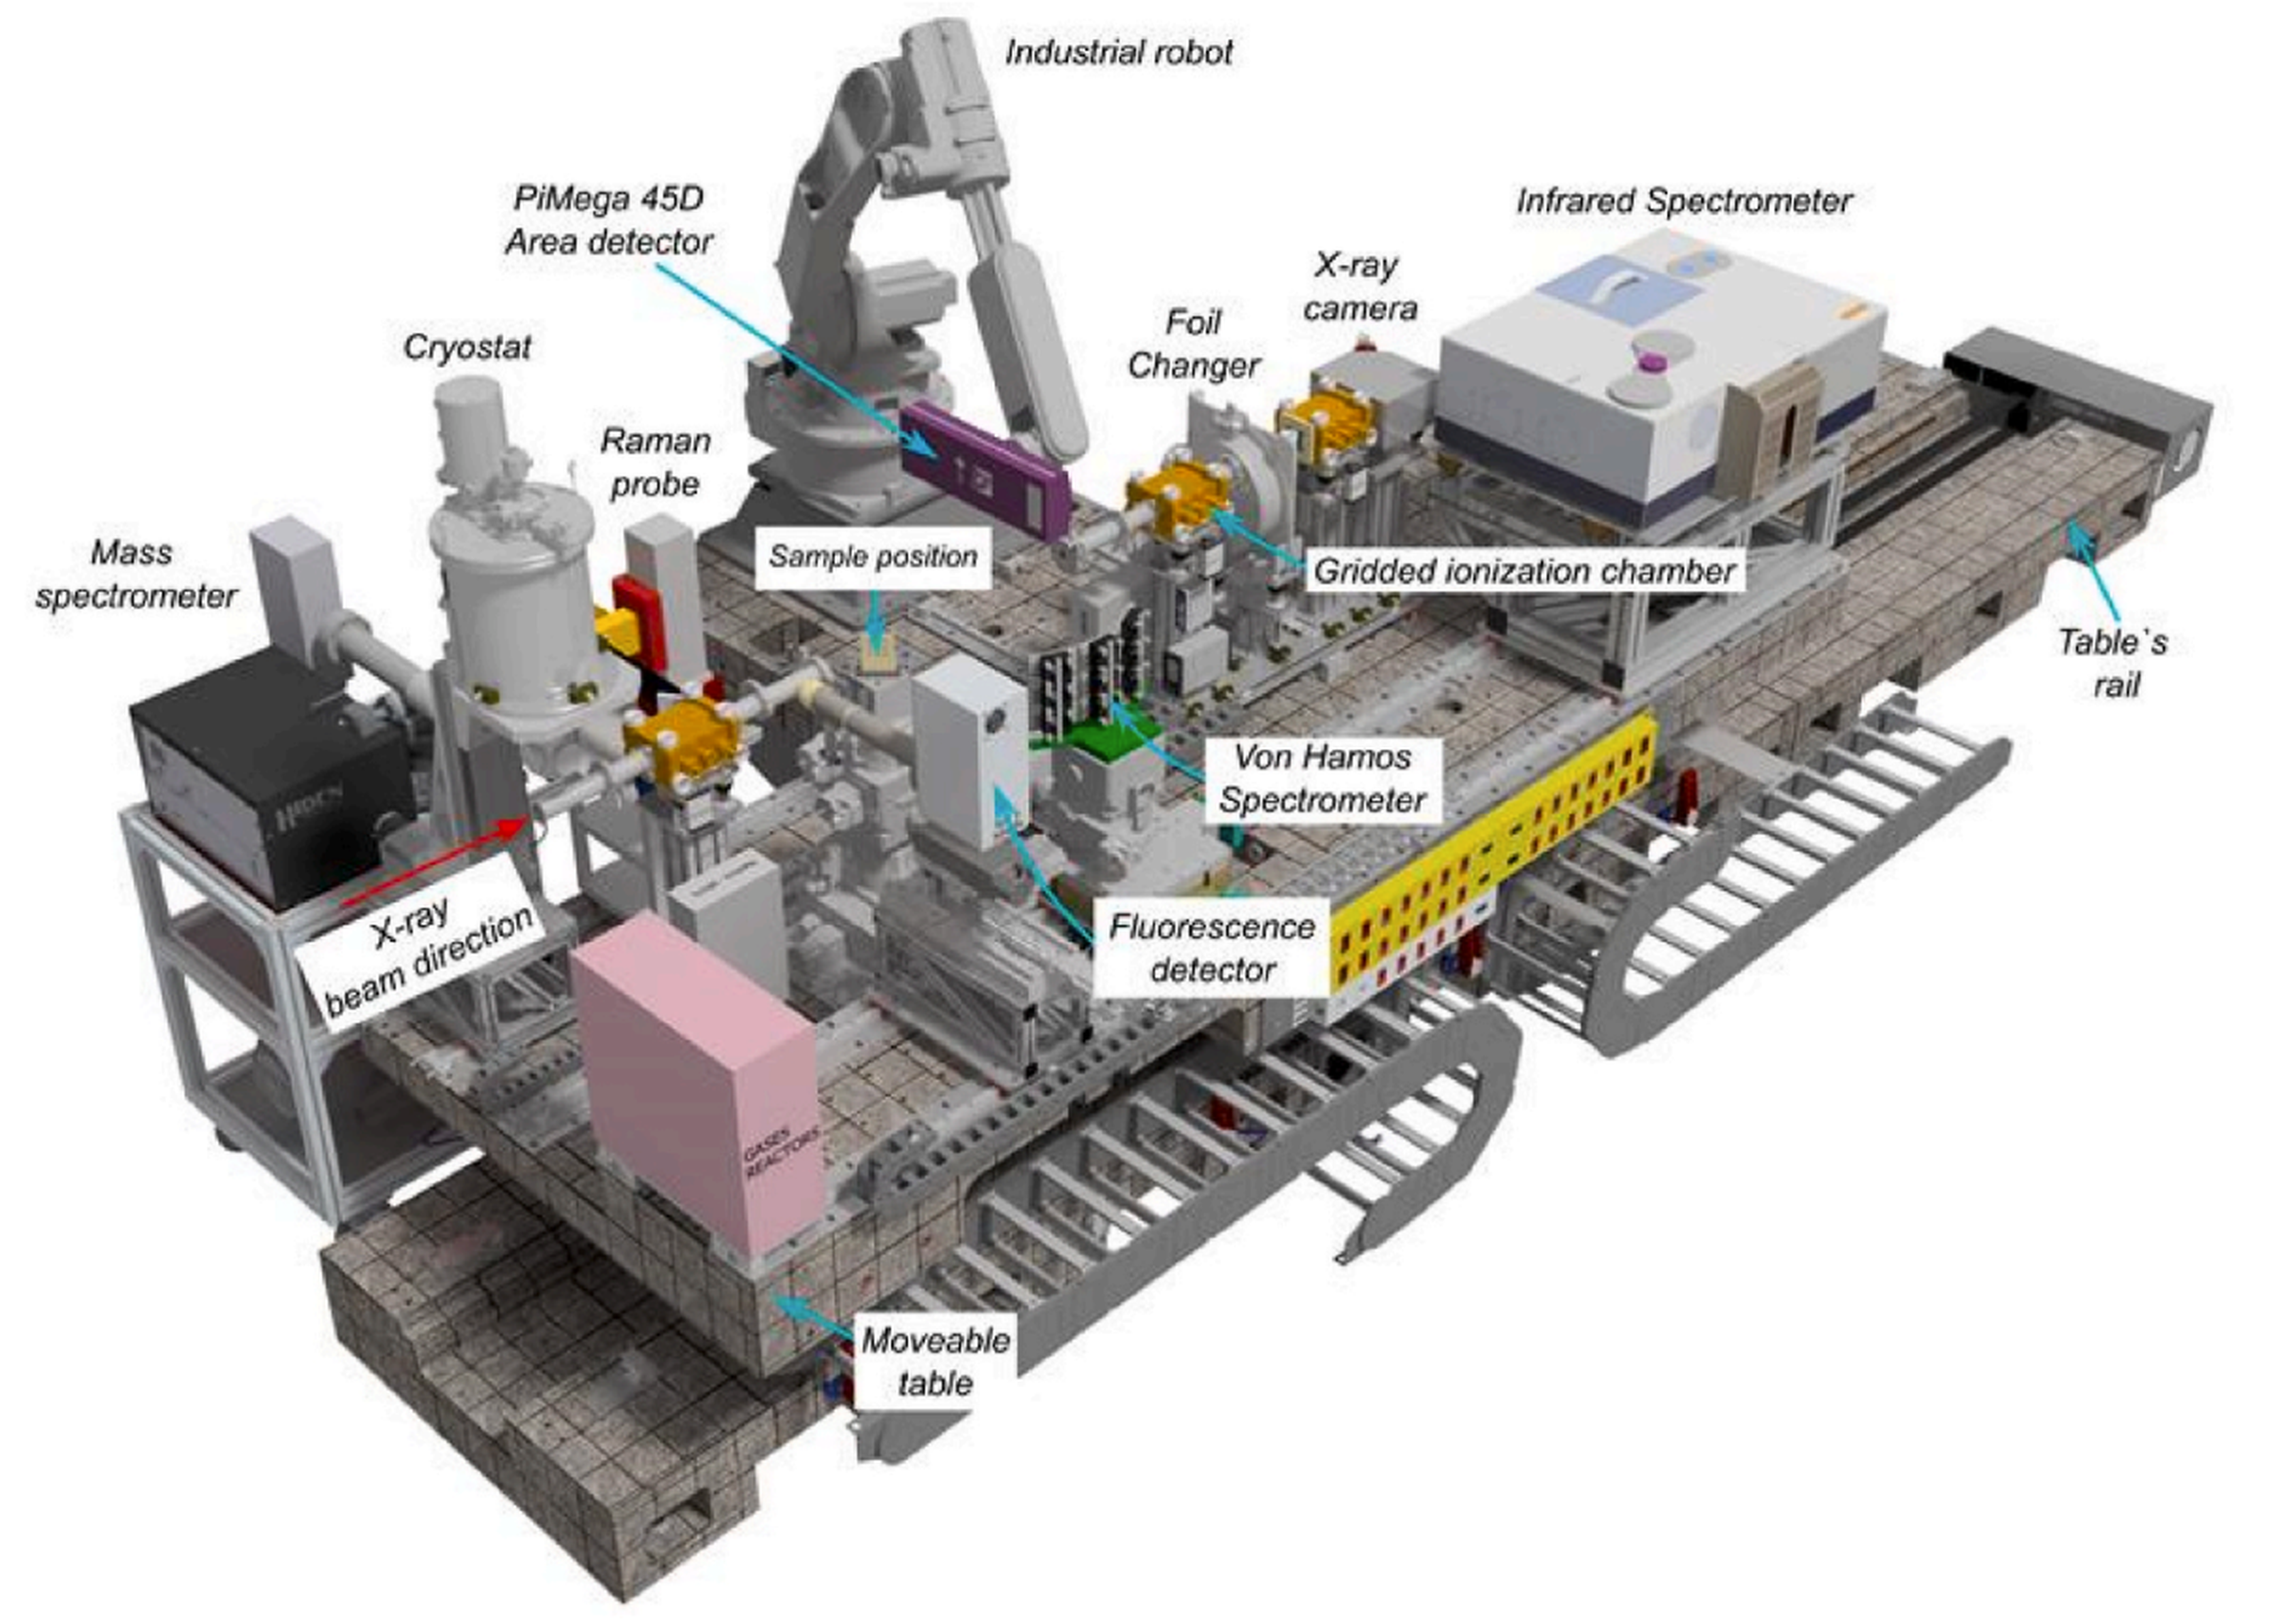
\includegraphics[width=.8\linewidth]{Figures/QUATI.png}
    \caption{Quati experimental beamline and subsystems. Figure reproduced from \cite{Santiago2023}.}
    \label{quati}
\end{figure}

The QUATI beamline has been designed to exploit the high brilliance of Sirius to perform rapid energy scans, enabling time-resolved XANES and EXAFS measurements on the millisecond to second timescale \cite{Santiago2023}. Such temporal resolution is critical for tracking redox oscillations, phase transitions, and active site changes during catalytic reactions and electrochemical processes.

The energy range of QUATI, extending from approximately 4.5 keV to 35 keV allows access to K edges of {\it 3d} transition metals and heavier elements, as well as the L edges of heavy elements. This spectral coverage is particularly relevant for materials based on nickel, cobalt, iron, copper, strontium, zirconium, yttrium, platinum, palladium, lanthanum, cerium, and gadolinium which are frequently employed in steam reforming of ethanol and solid oxide electrochemical devices.

In addition, the integration of innovative in-situ and operando electrochemical cells with QUATI spectroscopic capabilities is central to advancing the understanding of catalytic processes. These cells must fulfill several requirements. They must allow operation at high temperatures, often exceeding 800$^\circ$C for steam reforming and solid oxide electrochemical devices. They must withstand controlled gas atmospheres containing steam, ethanol, hydrogen, and oxygen. They must provide uniform temperature distribution, minimize X-ray absorption by cell components, and permit simultaneous complementary measurements such as electrochemical impedance spectroscopy (EIS). Furthermore, the cells must be designed to accommodate the beam path and scanning modes of the beamline, ensuring optimal signal-to-noise ratio and reproducibility.

For solid oxide fuel cells under operating conditions, the electrodes experience large oxygen chemical potential gradients \cite{Takashi2017}, thermal stress, and redox cycling. The local electronic structure of transition metal in these electrodes directly influences catalytic activity for oxygen reduction (ORR) and fuel oxidation reactions (HOR) \cite{Takashi2017,CHENG2023}. Operando XANES measurements at the Co, Fe, or Ni K edges allow quantification of valence state changes as a function of applied current density and gas composition. By integrating a custom-designed electrochemical cell compatible with high-temperature operation and X-ray fluorescence geometry \cite{Seval2021,Yoichiro2020}, one can measure the X-ray spectrum while the device is generating power.

The design of innovative electrochemical cells for synchrotron experiments requires optimization. The cell must maintain gas-tight separation between fuel and oxidant compartments while allowing X-ray photons to reach the electrode regions. Electrical contacts must withstand high temperatures without introducing significant X-ray absorption or scattering artifacts, and the geometry must ensure that the X-ray beam probes a representative volume of the electrode with minimal background contributions. At QUATI, the possibility of quick scanning enables the acquisition of sequential spectra during dynamic changes. This capability allows the correlation of structural changes with electrochemical performance in real time, offering insight into degradation mechanisms such as segregation, phase transition, or interfacial reactions \cite{Yao2019}.

For solid oxide electrolysis cells, operating in reverse mode to produce hydrogen, the scenario shares similar challenges and also similar operating conditions. For instance, operando XAS at the K or L edge under electrolysis conditions can quantify small shifts in edge position indicating changes in electronic structure associated with the processes \cite{Skinner2013}. Additionally, Time-resolved EXAFS can provide information on variations of the chemical bond length associated with oxygen non-stoichiometry changes during operation. By coupling these spectroscopic observations with electrochemical impedance data, it will become possible to distinguish between bulk and interfacial degradation pathways.

As illustrated in Figure \ref{methodology}, the research methodology enabled by QUATI in combination with in-situ cells extends beyond the empirical observation. The high resolution XANES and EXAFS data obtained under realistic conditions can be combined with density functional theory calculations to construct accurate structural models of catalytically active sites \cite{XU2024,Lucchetti2024}. By fitting experimental spectra with theoretically generated simulations, it will be possible to determine such structural information, guiding the selection of dopants, support compositions, and synthesis routes.

\begin{figure}[h]
    \centering
    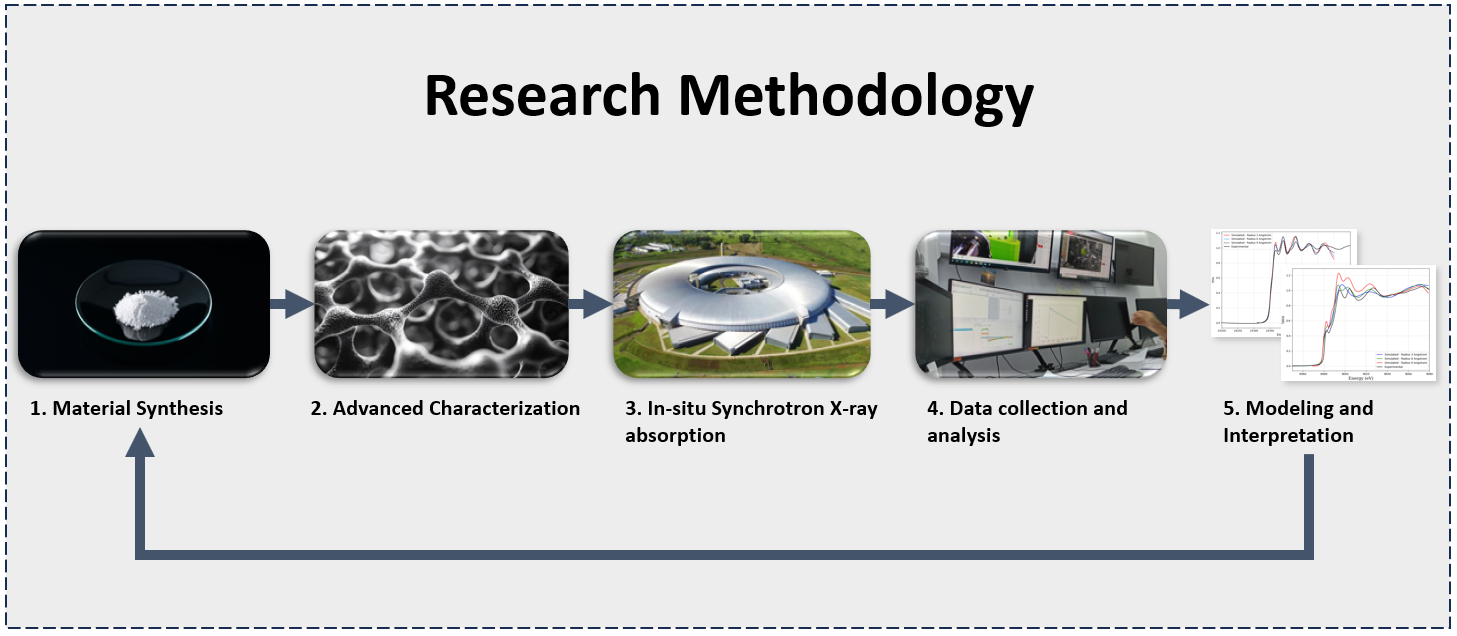
\includegraphics[width=1.\linewidth]{Figures/methodology.PNG}
    \caption{Figure showing a diagram illustrating the research methodology.}
    \label{methodology}
\end{figure}

The successful implementation of these research programs depends on the rigorous engineering of experimental infrastructure. Gas systems must deliver precisely controlled mixtures, temperature control must be accurate within a few degrees to avoid combination of thermal effects with intrinsic chemical changes. Data acquisition systems must synchronize X-ray scanning with external triggers to capture fast processes. Advanced data analysis pipelines, including principal component analysis, are required to deconvolute overlapping spectral features and identify distinct chemical species. The high photon flux at Sirius ensures that high signal-to-noise ratios can be achieved even under demanding conditions, enabling quantitative interpretation from the experiments.

%##########################
%\hl{START MODIFICATION}

Perturbed Angular Correlation Spectroscopy (PAC) will be employed to probe the local atomic and electronic environment of SOFC materials through hyperfine interactions, namely the magnetic hyperfine field (MHF) and electric field gradient (EFG), providing insights into crystal structure, defects, and local symmetry.

Experiments will be conducted at the Laboratory of Hyperfine Interactions (LIH) at IPEN (Brazil), which benefits from access to the IEA-R1 reactor for the production of radioactive probe nuclei (e.g., $^{111}$In, $^{181}$Hf). For this project, a newly implemented digital PAC spectrometer (figure \ref{pac}), based on LaBr$_3$ detectors and a CAEN acquisition system, will be used. This setup offers improved time resolution, higher counting efficiency, and faster data acquisition compared to conventional analog systems, allowing simultaneous analysis of multiple decay cascades and enhanced statistical reliability.

\begin{figure}[h]
    \centering
    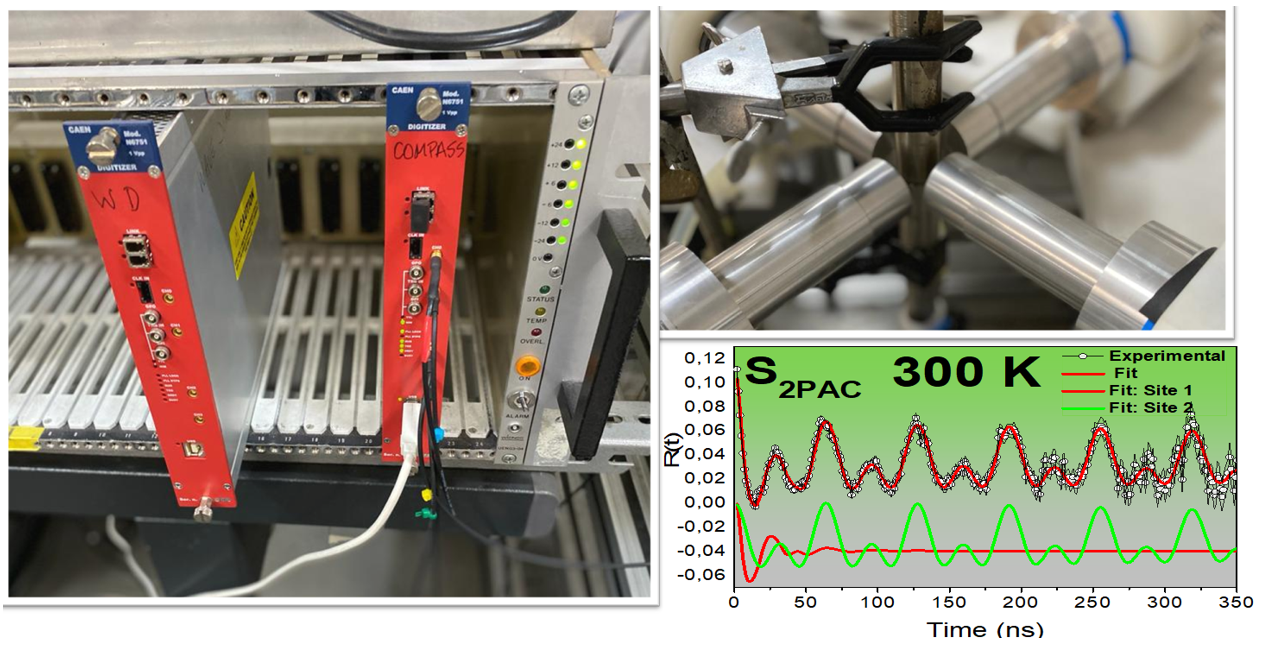
\includegraphics[width=1.\linewidth]{Figures/PAC.PNG}
    \caption{(a) Digital PAC spectrometer at LIH-IPEN; (b) furnace coupled to the digital spectrometer; and (c) characteristic PAC spectra of  $^{111}$In probe nuclei in a Ni-based catalyst.}
    \label{pac}
\end{figure}

Additionally, a dedicated high-temperature furnace enables in situ PAC measurements under controlled atmospheres, simulating realistic SOFC operating conditions. This capability allows the investigation of temperature-dependent phenomena such as defect dynamics, oxygen vacancy behavior, and phase stability, providing a comprehensive understanding of structure–property relationships under operando conditions.


%\hl{END MODIFICATION}
%##########################

In summary, the convergence of high-brilliance synchrotron radiation at Sirius, advanced X-ray absorption spectroscopy at the QUATI beamline, and purpose built innovative in-situ and operando cells establishes a framework for investigating catalytic materials for ethanol steam reforming and solid oxide electrochemical devices. The ability to probe local atomic structure and electronic configuration under realistic conditions, with high temporal and spatial resolution, addresses a longstanding gap in catalysis and electrochemistry research. Through rigorous integration of spectroscopic analysis, and theoretical modeling, this approach enables the development of next-generation materials with improved activity, stability, and sustainability. The scientific and technological implications extend from fundamental understanding of the chemical reaction dynamics to practical deployment of renewable energy systems, positioning this research at the forefront of advanced energy materials science.